\chapter{Understanding VPNs: From Theory to Practice}

This chapter provides a comprehensive deep dive into Virtual Private Networks (VPNs), exploring how they work at different layers of the network stack, the protocols they use, and how they integrate with system networking. This knowledge is essential for understanding why endpoint testing requires multiple approaches and how Smart Relay orchestrates VPN connections.

\section{What is a VPN?}

A Virtual Private Network (VPN) creates a secure, encrypted tunnel between your device and a remote server, making it appear as if your network traffic originates from the VPN server rather than your actual location. This provides:

\begin{itemize}
    \item \textbf{Privacy}: Your real IP address is hidden from websites and services.
    \item \textbf{Security}: Traffic is encrypted, protecting it from interception.
    \item \textbf{Geographic flexibility}: Access content restricted to specific regions.
    \item \textbf{Network isolation}: Create private networks over public infrastructure.
\end{itemize}

\section{The OSI Model and VPN Layers}

VPNs operate at multiple layers of the OSI (Open Systems Interconnection) model. Understanding these layers helps diagnose connection issues and design better testing strategies.

\subsection{Layer 1-2: Physical and Data Link}

At the lowest layers, VPNs don't directly operate, but they rely on:
\begin{itemize}
    \item \textbf{Physical Layer (Layer 1)}: The actual network cables, wireless signals, and hardware.
    \item \textbf{Data Link Layer (Layer 2)}: Ethernet frames, MAC addresses, and local network protocols.
\end{itemize}

VPNs typically start their work at Layer 3 (Network) or higher.

\subsection{Layer 3: Network Layer (IP)}

The Network Layer is where IP (Internet Protocol) operates. This is where routing decisions are made and where many VPN protocols begin their work.

\begin{figure}[h]
    \centering
    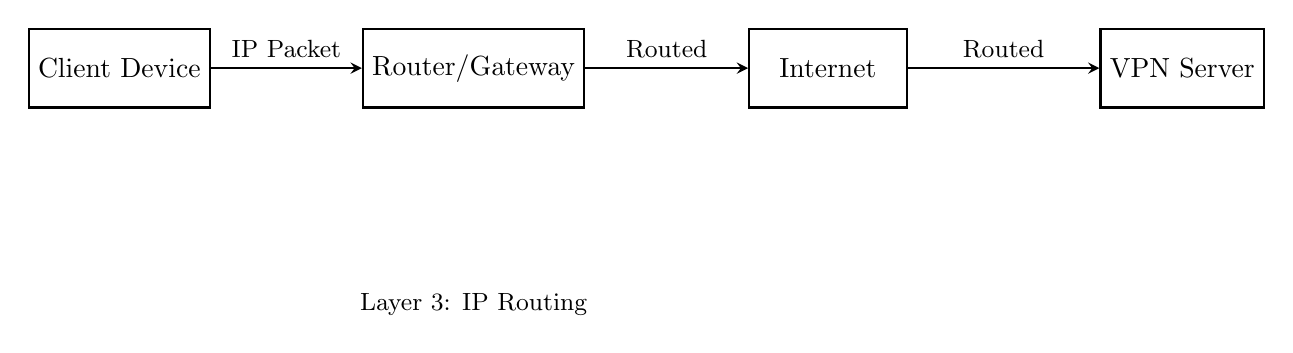
\begin{tikzpicture}[node distance=2.5cm,>=stealth,thick]
        \node (client) [draw, rectangle, minimum width=2cm, minimum height=1cm] {Client Device};
        \node (router) [draw, rectangle, minimum width=2cm, minimum height=1cm, right of=client, xshift=2cm] {Router/Gateway};
        \node (internet) [draw, rectangle, minimum width=2cm, minimum height=1cm, right of=router, xshift=2cm] {Internet};
        \node (vpn) [draw, rectangle, minimum width=2cm, minimum height=1cm, right of=internet, xshift=2cm] {VPN Server};
        
        \draw[->] (client) -- node[above]{\small IP Packet} (router);
        \draw[->] (router) -- node[above]{\small Routed} (internet);
        \draw[->] (internet) -- node[above]{\small Routed} (vpn);
        
        \node [below of=router, yshift=-0.5cm] {\small Layer 3: IP Routing};
    \end{tikzpicture}
    \caption{Network Layer (Layer 3) routing without VPN.}
\end{figure}

\textbf{Key concepts:}
\begin{itemize}
    \item \textbf{IP Addresses}: Unique identifiers for devices on the network (e.g., 192.168.1.100, 8.8.8.8).
    \item \textbf{Routing}: The process of forwarding packets from source to destination.
    \item \textbf{Subnetting}: Dividing networks into smaller subnetworks.
    \item \textbf{ICMP}: Internet Control Message Protocol for error reporting and diagnostics (ping uses ICMP).
\end{itemize}

\subsection{Layer 4: Transport Layer (TCP/UDP)}

The Transport Layer provides end-to-end communication services. This is where TCP (Transmission Control Protocol) and UDP (User Datagram Protocol) operate.

\begin{figure}[h]
    \centering
    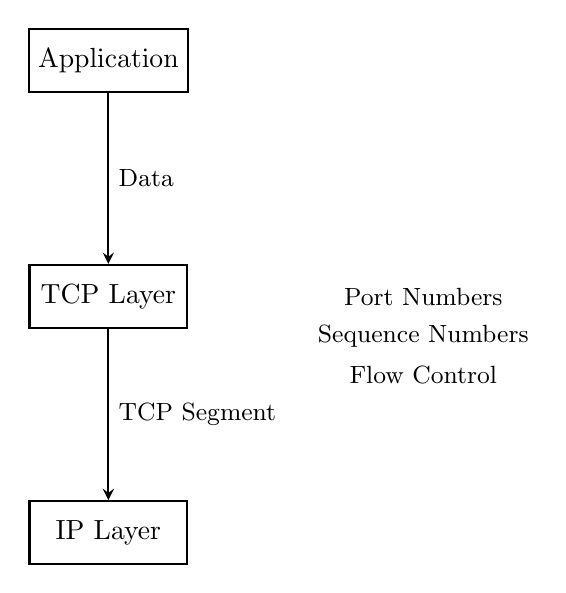
\begin{tikzpicture}[node distance=3cm,>=stealth,thick]
        \node (app) [draw, rectangle, minimum width=2cm, minimum height=0.8cm] {Application};
        \node (tcp) [draw, rectangle, minimum width=2cm, minimum height=0.8cm, below of=app] {TCP Layer};
        \node (ip) [draw, rectangle, minimum width=2cm, minimum height=0.8cm, below of=tcp] {IP Layer};
        
        \draw[->] (app) -- node[right]{\small Data} (tcp);
        \draw[->] (tcp) -- node[right]{\small TCP Segment} (ip);
        
        \node [right of=tcp, xshift=1cm] {\small Port Numbers};
        \node [right of=tcp, xshift=1cm, yshift=-0.5cm] {\small Sequence Numbers};
        \node [right of=tcp, xshift=1cm, yshift=-1cm] {\small Flow Control};
    \end{tikzpicture}
    \caption{Transport Layer (Layer 4) adds port numbers and reliability.}
\end{figure}

\textbf{TCP Three-Way Handshake:}
\begin{enumerate}
    \item \textbf{SYN}: Client sends a synchronization packet with a random sequence number.
    \item \textbf{SYN-ACK}: Server responds with its own sequence number and acknowledges the client's.
    \item \textbf{ACK}: Client acknowledges the server's sequence number. Connection established.
\end{enumerate}

\begin{figure}[h]
    \centering
    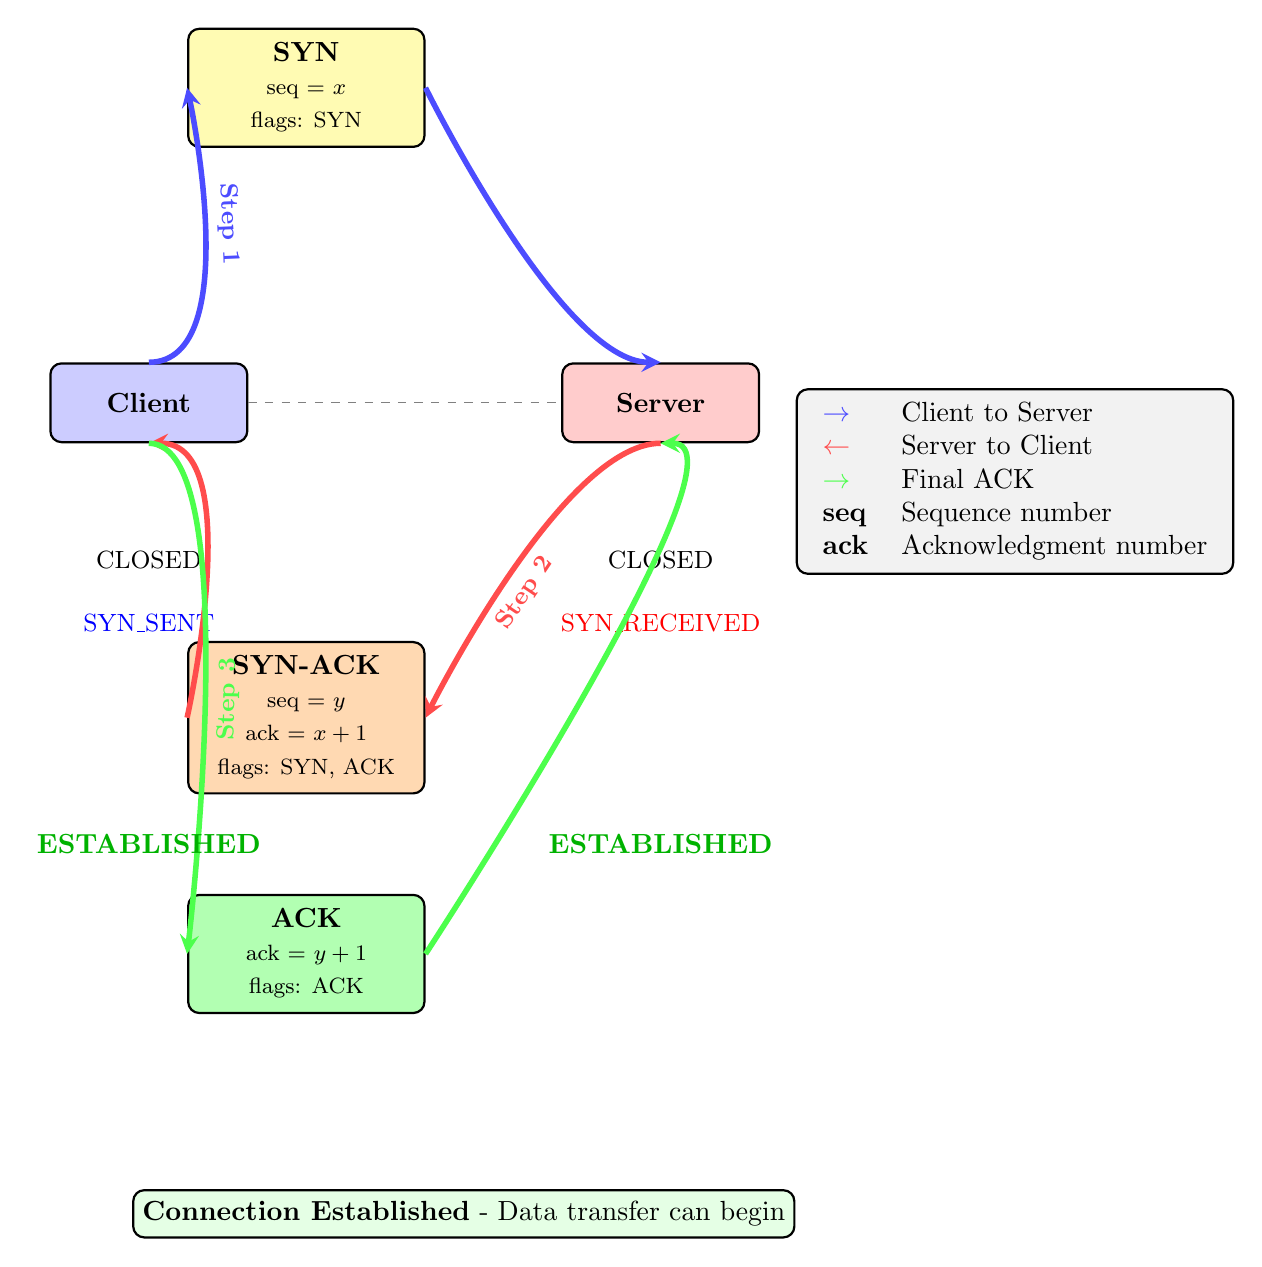
\begin{tikzpicture}[
        node distance=2.5cm,
        >=stealth,
        thick,
        state/.style={draw, rectangle, rounded corners, minimum width=2.5cm, minimum height=1cm, fill=blue!10},
        packet/.style={draw, rectangle, rounded corners, minimum width=3cm, minimum height=0.8cm, fill=green!20},
        arrow/.style={->, line width=2pt},
        timeline/.style={dashed, gray, line width=0.5pt}
    ]
        % Client and Server nodes
        \node (client) [state, fill=blue!20] {\textbf{Client}};
        \node (server) [state, fill=red!20, right of=client, xshift=4cm] {\textbf{Server}};
        
        % Connection states
        \node (client_closed) [below of=client, yshift=0.5cm, font=\small] {CLOSED};
        \node (server_closed) [below of=server, yshift=0.5cm, font=\small] {CLOSED};
        
        % Timeline
        \draw[timeline] (client) -- (server);
        
        % Step 1: SYN
        \node (syn_packet) [packet, fill=yellow!30, above of=client, yshift=1.5cm, xshift=2cm] {
            \begin{tabular}{c}
                \textbf{SYN} \\
                \footnotesize seq = $x$ \\
                \footnotesize flags: SYN
            \end{tabular}
        };
        \draw[arrow, blue!70] (client.north) .. controls (client.north east) and (syn_packet.west) .. 
            node[above, sloped, font=\small] {\textbf{Step 1}} (syn_packet.west);
        \draw[arrow, blue!70] (syn_packet.east) .. controls (syn_packet.east) and (server.north west) .. (server.north);
        
        \node (client_syn_sent) [below of=client, yshift=-0.3cm, font=\small, text=blue] {SYN\_SENT};
        
        % Step 2: SYN-ACK
        \node (synack_packet) [packet, fill=orange!30, below of=client, yshift=-1.5cm, xshift=2cm] {
            \begin{tabular}{c}
                \textbf{SYN-ACK} \\
                \footnotesize seq = $y$ \\
                \footnotesize ack = $x+1$ \\
                \footnotesize flags: SYN, ACK
            \end{tabular}
        };
        \draw[arrow, red!70] (server.south) .. controls (server.south west) and (synack_packet.east) .. 
            node[below, sloped, font=\small] {\textbf{Step 2}} (synack_packet.east);
        \draw[arrow, red!70] (synack_packet.west) .. controls (synack_packet.west) and (client.south east) .. (client.south);
        
        \node (server_syn_rcvd) [below of=server, yshift=-0.3cm, font=\small, text=red] {SYN\_RECEIVED};
        
        % Step 3: ACK
        \node (ack_packet) [packet, fill=green!30, below of=synack_packet, yshift=-0.5cm] {
            \begin{tabular}{c}
                \textbf{ACK} \\
                \footnotesize ack = $y+1$ \\
                \footnotesize flags: ACK
            \end{tabular}
        };
        \draw[arrow, green!70] (client.south) .. controls (client.south east) and (ack_packet.west) .. 
            node[below, sloped, font=\small] {\textbf{Step 3}} (ack_packet.west);
        \draw[arrow, green!70] (ack_packet.east) .. controls (ack_packet.east) and (server.south east) .. (server.south);
        
        % Established state
        \node (client_est) [below of=client_syn_sent, yshift=-0.3cm, font=\small, text=green!70!black, font=\bfseries] {ESTABLISHED};
        \node (server_est) [below of=server_syn_rcvd, yshift=-0.3cm, font=\small, text=green!70!black, font=\bfseries] {ESTABLISHED};
        
        % Connection established indicator
        \node (established) [draw, rectangle, rounded corners, fill=green!10, minimum width=6cm, minimum height=0.6cm, 
            below of=ack_packet, yshift=-0.8cm, xshift=2cm] {
            \textbf{Connection Established} - Data transfer can begin
        };
        
        % Legend
        \node (legend) [draw, rectangle, rounded corners, fill=gray!10, minimum width=5cm, minimum height=2cm,
            right of=server, xshift=2cm, yshift=-1cm] {
            \begin{tabular}{ll}
                \textcolor{blue!70}{$\rightarrow$} & Client to Server \\
                \textcolor{red!70}{$\leftarrow$} & Server to Client \\
                \textcolor{green!70}{$\rightarrow$} & Final ACK \\
                \textbf{seq} & Sequence number \\
                \textbf{ack} & Acknowledgment number \\
            \end{tabular}
        };
    \end{tikzpicture}
    \caption{TCP three-way handshake process with detailed packet information and state transitions.}
\end{figure}
\textbf{Why this matters for VPN testing:}
\begin{itemize}
    \item If SYN packets are sent but no SYN-ACK is received, the connection fails at Layer 4.
    \item Firewalls often drop SYN packets silently (stealth mode), causing timeouts.
    \item Connection refused errors indicate the port is closed (RST packet received).
    \item Timeouts suggest packets are being dropped or not routed correctly.
\end{itemize}

\subsection{Layer 5-7: Session, Presentation, Application}

Higher layers handle:
\begin{itemize}
    \item \textbf{Session Layer (Layer 5)}: Manages sessions between applications.
    \item \textbf{Presentation Layer (Layer 6)}: Data translation, encryption, compression.
    \item \textbf{Application Layer (Layer 7)}: HTTP, HTTPS, DNS, FTP, and application protocols.
\end{itemize}

VPN protocols often operate at these layers, encapsulating lower-layer traffic.

\section{VPN Tunneling Mechanisms}

VPNs create "tunnels" by encapsulating one protocol within another. This section explains the different tunneling approaches.

\subsection{IP-in-IP Tunneling}

The simplest form of tunneling: one IP packet is placed inside another IP packet.

\begin{figure}[h]
    \centering
    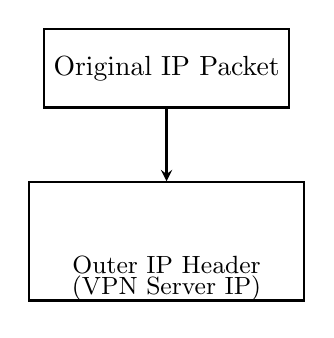
\begin{tikzpicture}[node distance=2cm,>=stealth,thick]
        \node (original) [draw, rectangle, minimum width=3cm, minimum height=1cm] {Original IP Packet};
        \node (encapsulated) [draw, rectangle, minimum width=3.5cm, minimum height=1.5cm, below of=original, yshift=-0.2cm] {};
        \node [below of=original, yshift=-0.5cm] {\small Outer IP Header};
        \node [below of=original, yshift=-0.8cm] {\small (VPN Server IP)};
        
        \draw[->] (original) -- (encapsulated);
    \end{tikzpicture}
    \caption{IP-in-IP encapsulation: original packet wrapped in new IP header.}
\end{figure}

\textbf{How it works:}
\begin{enumerate}
    \item Original packet has destination IP of the final target.
    \item VPN client wraps it in a new IP packet with destination of VPN server.
    \item VPN server unwraps and forwards the original packet.
    \item Response follows the reverse path.
\end{enumerate}

\subsection{Protocol-Specific Tunneling}

Different VPN protocols use different encapsulation methods:

\subsubsection{OpenVPN}
\begin{itemize}
    \item Uses UDP or TCP for transport.
    \item Encapsulates IP packets in OpenVPN protocol.
    \item Supports both TUN (Layer 3) and TAP (Layer 2) modes.
    \item Uses TLS/SSL for key exchange and authentication.
\end{itemize}

\subsubsection{WireGuard}
\begin{itemize}
    \item Modern, lightweight VPN protocol.
    \item Uses UDP for transport.
    \item Operates at Layer 3 (IP level).
    \item Uses state-of-the-art cryptography (ChaCha20, Poly1305, Curve25519).
\end{itemize}

\subsubsection{IPSec}
\begin{itemize}
    \item Operates at Layer 3 (Network Layer).
    \item Can work in two modes:
    \begin{itemize}
        \item \textbf{Transport Mode}: Encrypts only the payload.
        \item \textbf{Tunnel Mode}: Encrypts the entire IP packet.
    \end{itemize}
    \item Often used for site-to-site VPNs.
\end{itemize}

\subsubsection{Shadowsocks, VMess, VLESS (Proxy Protocols)}
\begin{itemize}
    \item These are proxy protocols, not traditional VPNs.
    \item Operate at Layer 5-7 (Application/Session layers).
    \item Encrypt and forward application-layer traffic (HTTP, HTTPS, etc.).
    \item Don't create a true network interface like traditional VPNs.
    \item Work by intercepting application traffic and forwarding it through a proxy server.
\end{itemize}

\section{How VPNs Integrate with Operating Systems}

Understanding how VPNs hook into the operating system is crucial for implementing system proxy integration.

\subsection{Network Interface Creation}

Traditional VPNs create virtual network interfaces:

\begin{figure}[h]
    \centering
    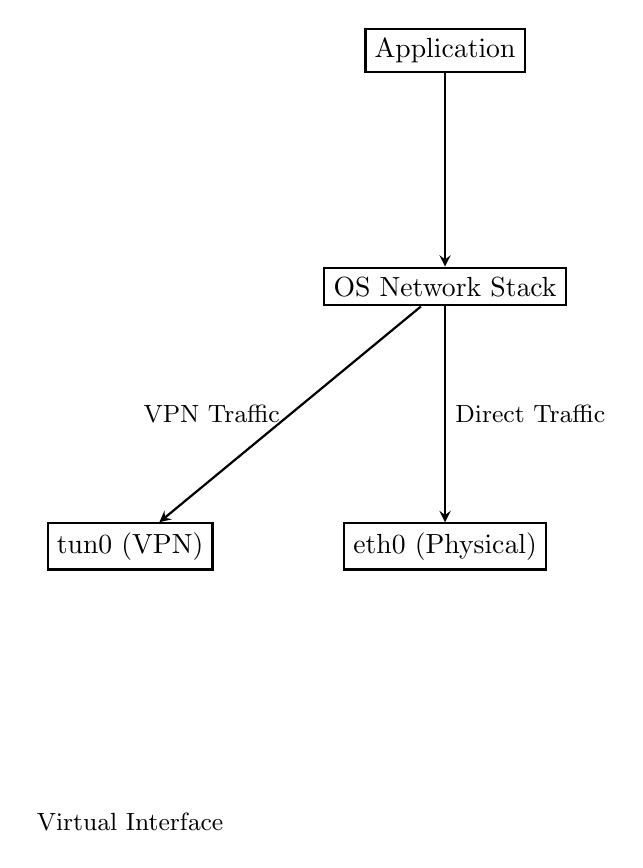
\begin{tikzpicture}[node distance=3cm,>=stealth,thick]
        \node (app) [draw, rectangle, minimum width=2cm] {Application};
        \node (os) [draw, rectangle, minimum width=2cm, below of=app] {OS Network Stack};
        \node (eth0) [draw, rectangle, minimum width=2cm, below of=os, yshift=-0.3cm] {eth0 (Physical)};
        \node (tun0) [draw, rectangle, minimum width=2cm, left of=eth0, xshift=-1cm] {tun0 (VPN)};
        
        \draw[->] (app) -- (os);
        \draw[->] (os) -- node[left]{\small VPN Traffic} (tun0);
        \draw[->] (os) -- node[right]{\small Direct Traffic} (eth0);
        
        \node [below of=tun0, yshift=-0.5cm] {\small Virtual Interface};
    \end{tikzpicture}
    \caption{VPN creates virtual network interface (tun0/tap0).}
\end{figure}

\textbf{On different operating systems:}
\begin{itemize}
    \item \textbf{Linux}: Creates \texttt{tun0} or \texttt{tap0} interfaces.
    \item \textbf{Windows}: Creates TAP adapters (visible in Network Connections).
    \item \textbf{macOS}: Creates \texttt{utun} interfaces.
\end{itemize}

\subsection{Routing Table Modification}

VPNs modify the routing table to direct traffic through the VPN interface:

\begin{verbatim}
# Example routing table with VPN active
Destination     Gateway         Genmask         Flags Interface
0.0.0.0         10.8.0.1        0.0.0.0         UG    tun0    # Default via VPN
10.8.0.0        0.0.0.0         255.255.255.0   U     tun0    # VPN subnet
192.168.1.0     0.0.0.0         255.255.255.0   U     eth0    # Local network
\end{verbatim}

\subsection{Proxy vs. VPN: System Integration}

\subsubsection{Traditional VPN (TUN/TAP)}
\begin{itemize}
    \item Creates a virtual network interface.
    \item Modifies routing table.
    \item All IP traffic can be routed through VPN.
    \item Transparent to applications (they don't know VPN exists).
    \item Examples: OpenVPN, WireGuard, IPSec.
\end{itemize}

\subsubsection{Proxy-Based (Application Layer)}
\begin{itemize}
    \item No virtual network interface.
    \item Applications must be configured to use proxy.
    \item Only configured applications use proxy.
    \item System proxy settings tell applications where to connect.
    \item Examples: Shadowsocks, VMess, VLESS, SOCKS5, HTTP proxy.
\end{itemize}

\begin{figure}[h]
    \centering
    \begin{tikzpicture}[node distance=3cm,>=stealth,thick]
        \node (app1) [draw, rectangle, minimum width=1.5cm] {App 1};
        \node (app2) [draw, rectangle, minimum width=1.5cm, below of=app1] {App 2};
        \node (proxy) [draw, rectangle, minimum width=2cm, right of=app1, xshift=1cm] {Proxy Client};
        \node (server) [draw, rectangle, minimum width=2cm, right of=proxy, xshift=1cm] {Proxy Server};
        
        \draw[->] (app1) -- node[above]{\small Configured} (proxy);
        \draw[->] (app2) -- node[below]{\small Direct} ++(2,0);
        \draw[->] (proxy) -- node[above]{\small Encrypted} (server);
        
        \node [below of=app2, yshift=-0.5cm] {\small Not using proxy};
    \end{tikzpicture}
    \caption{Proxy-based VPN: only configured applications use it.}
\end{figure}

\section{Windows System Proxy Integration}

Smart Relay uses Windows system proxy settings to route application traffic through proxy servers. Understanding how this works is essential.

\subsection{Windows Proxy Registry Keys}

Windows stores proxy settings in the registry:

\begin{verbatim}
HKEY_CURRENT_USER\Software\Microsoft\Windows\CurrentVersion\Internet Settings
\end{verbatim}

\textbf{Key values:}
\begin{itemize}
    \item \texttt{ProxyEnable}: 1 = proxy enabled, 0 = disabled.
    \item \texttt{ProxyServer}: Format: \texttt{host:port} or \texttt{http=host:port;https=host:port;ftp=host:port;socks=host:port}
    \item \texttt{ProxyOverride}: Semicolon-separated list of addresses that bypass proxy.
    \item \texttt{AutoConfigURL}: URL to PAC (Proxy Auto-Configuration) script.
\end{itemize}

\subsection{Global Proxy Mode}

In Global mode, all HTTP/HTTPS traffic goes through the specified proxy:

\begin{figure}[h]
    \centering
    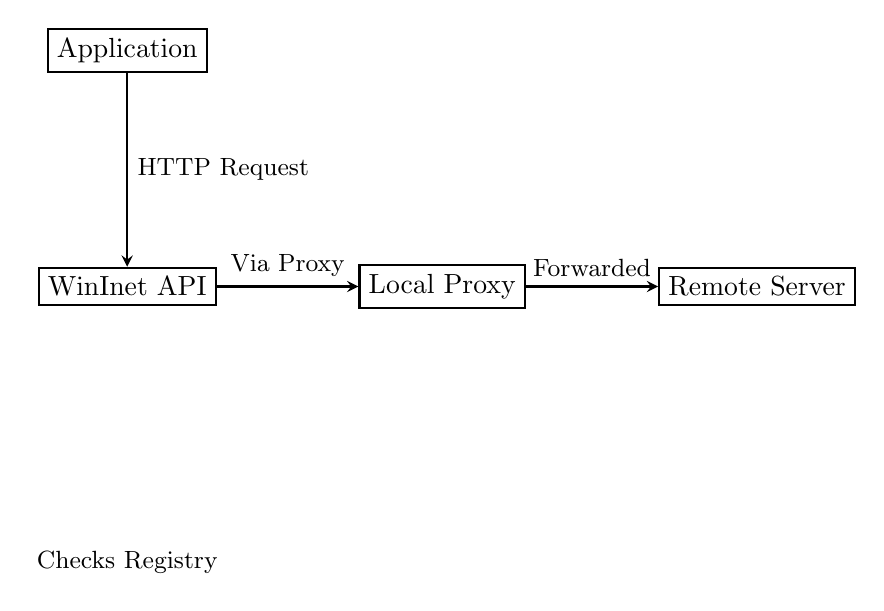
\begin{tikzpicture}[node distance=3cm,>=stealth,thick]
        \node (app) [draw, rectangle, minimum width=2cm] {Application};
        \node (wininet) [draw, rectangle, minimum width=2cm, below of=app] {WinInet API};
        \node (proxy) [draw, rectangle, minimum width=2cm, right of=wininet, xshift=1cm] {Local Proxy};
        \node (server) [draw, rectangle, minimum width=2cm, right of=proxy, xshift=1cm] {Remote Server};
        
        \draw[->] (app) -- node[right]{\small HTTP Request} (wininet);
        \draw[->] (wininet) -- node[above]{\small Via Proxy} (proxy);
        \draw[->] (proxy) -- node[above]{\small Forwarded} (server);
        
        \node [below of=wininet, yshift=-0.5cm] {\small Checks Registry};
    \end{tikzpicture}
    \caption{Global proxy mode: WinInet routes all HTTP/HTTPS through proxy.}
\end{figure}

\textbf{How it works:}
\begin{enumerate}
    \item Application makes HTTP/HTTPS request using WinInet API.
    \item WinInet checks registry for \texttt{ProxyEnable} and \texttt{ProxyServer}.
    \item If enabled, WinInet connects to proxy instead of destination.
    \item Proxy forwards request to actual destination.
    \item Response follows reverse path.
\end{enumerate}

\subsection{PAC (Proxy Auto-Configuration) Mode}

PAC mode uses a JavaScript file to dynamically determine proxy settings:

\begin{verbatim}
function FindProxyForURL(url, host) {
    if (isPlainHostName(host) || 
        dnsDomainIs(host, ".local") ||
        isInNet(host, "192.168.0.0", "255.255.0.0")) {
        return "DIRECT";
    }
    return "PROXY 127.0.0.1:1080; SOCKS5 127.0.0.1:1080";
}
\end{verbatim}

\textbf{Benefits:}
\begin{itemize}
    \item Different proxies for different domains.
    \item Bypass proxy for local addresses.
    \item Load balancing across multiple proxies.
    \item Dynamic configuration without registry changes.
\end{itemize}

\subsection{Limitations of System Proxy}

\begin{itemize}
    \item \textbf{Application support}: Only applications using WinInet API respect system proxy.
    \item \textbf{Non-HTTP traffic}: System proxy typically only handles HTTP/HTTPS, not raw TCP/UDP.
    \item \textbf{Administrator rights}: Some proxy operations may require elevated privileges.
    \item \textbf{Bypass mechanisms}: Some applications have hardcoded proxy bypasses.
\end{itemize}

\section{Why Endpoint Testing is Complex}

Now that we understand VPNs and networking layers, we can see why comprehensive endpoint testing requires multiple approaches.

\subsection{The Testing Challenge}

When testing a VPN endpoint, we need to verify:

\begin{enumerate}
    \item \textbf{DNS Resolution (Layer 7)}: Can we resolve the hostname?
    \item \textbf{Network Reachability (Layer 3)}: Can we route packets to the server?
    \item \textbf{Port Accessibility (Layer 4)}: Is the port open and accepting connections?
    \item \textbf{Protocol Compatibility (Layer 5-7)}: Does the protocol work correctly?
    \item \textbf{Proxy Functionality (Layer 5-7)}: Can we actually use it as a proxy?
\end{enumerate}

\subsection{Why Direct TCP Tests May Fail}

A direct TCP connection test might fail even if the endpoint works through a proxy:

\begin{itemize}
    \item \textbf{Firewall blocking}: The server may only accept connections from specific IPs (e.g., only from other VPN servers).
    \item \textbf{Protocol requirement}: Some protocols (like VMess) require specific handshakes that a simple TCP test can't perform.
    \item \textbf{Rate limiting}: Servers may rate-limit direct connections but allow proxy connections.
    \item \textbf{Geographic restrictions}: The server may block direct connections from certain regions.
\end{itemize}

\subsection{Why Proxy Tests May Fail}

Testing through a local proxy may also fail:

\begin{itemize}
    \item \textbf{Local proxy not running}: The proxy client (xray, sing-box) must be running and configured.
    \item \textbf{Configuration mismatch}: The proxy client may not be configured to use the endpoint being tested.
    \item \textbf{Protocol incompatibility}: The local proxy may not support the endpoint's protocol.
    \item \textbf{Authentication failure}: Credentials or encryption keys may be incorrect.
\end{itemize}

\subsection{Smart Testing Strategy}

Smart Relay's comprehensive testing approach:

\begin{enumerate}
    \item \textbf{DNS Resolution}: Verify hostname can be resolved (Layer 7).
    \item \textbf{Direct TCP Connection}: Attempt direct connection (Layer 4).
    \begin{itemize}
        \item If successful: Endpoint is reachable.
        \item If failed: May still work through proxy.
    \end{itemize}
    \item \textbf{Proxy-Based Test}: If local proxy is available, test through it (Layer 5-7).
    \item \textbf{Extended Timeout}: Some connections are slow but work (Layer 4).
    \item \textbf{Diagnostic Analysis}: Categorize failures to provide actionable feedback.
\end{enumerate}

\section{Packet-Level Analysis}

Understanding what happens at the packet level helps diagnose connection issues.

\subsection{TCP Packet Structure}

A TCP packet contains:

\begin{verbatim}
+-------------------+-------------------+
| Source Port (16)  | Dest Port (16)    |
+-------------------+-------------------+
| Sequence Number (32 bits)              |
+---------------------------------------+
| Acknowledgment Number (32 bits)       |
+-------+-------+-----------------------+
| Data  | Flags | Window Size (16)      |
|Offset |(SYN,  |                       |
| (4)   |ACK...)|                       |
+-------+-------+-----------------------+
| Checksum (16)    | Urgent Pointer (16)|
+------------------+--------------------+
| Options (variable length)             |
+---------------------------------------+
| Data (variable length)                |
+---------------------------------------+
\end{verbatim}

\subsection{Connection States}

TCP connections go through several states:

\begin{itemize}
    \item \textbf{CLOSED}: No connection exists.
    \item \textbf{SYN\_SENT}: Client sent SYN, waiting for SYN-ACK.
    \item \textbf{SYN\_RECEIVED}: Server received SYN, sent SYN-ACK, waiting for ACK.
    \item \textbf{ESTABLISHED}: Connection is open and data can be exchanged.
    \item \textbf{FIN\_WAIT}: Connection is being closed.
    \item \textbf{CLOSED}: Connection is fully closed.
\end{itemize}

\subsection{Error Scenarios}

\begin{itemize}
    \item \textbf{Connection Refused (RST)}:
    \begin{itemize}
        \item Server received SYN.
        \item Server sent RST (reset) packet.
        \item Port is closed or service not running.
    \end{itemize}
    
    \item \textbf{Connection Timeout}:
    \begin{itemize}
        \item Client sent SYN.
        \item No response received (SYN-ACK or RST).
        \item Firewall dropping packets silently.
        \item Network routing issue.
        \item Server is down or unreachable.
    \end{itemize}
    
    \item \textbf{Network Unreachable}:
    \begin{itemize}
        \item No route to destination.
        \item ICMP "Destination Unreachable" may be received.
        \item Network configuration issue.
    \end{itemize}
\end{itemize}

\section{Practical Implications for Smart Relay}

This deep understanding of VPNs and networking informs Smart Relay's design:

\begin{itemize}
    \item \textbf{Multi-layer testing}: Test at DNS, TCP, and proxy levels.
    \item \textbf{Comprehensive diagnostics}: Provide detailed information about failures.
    \item \textbf{System integration}: Use Windows registry for proxy configuration.
    \item \textbf{Protocol support}: Handle both traditional VPNs and proxy protocols.
    \item \textbf{Error categorization}: Help users understand what went wrong.
\end{itemize}

\section{Understanding Network Censorship and Firewalls}

Understanding how network firewalls and censorship systems work helps explain why endpoints may fail even when you're outside restricted regions. This section discusses the technical principles behind network filtering systems.

\subsection{Multi-Layer Filtering}

Network filtering systems can operate at multiple OSI layers:

\begin{figure}[h]
    \centering
    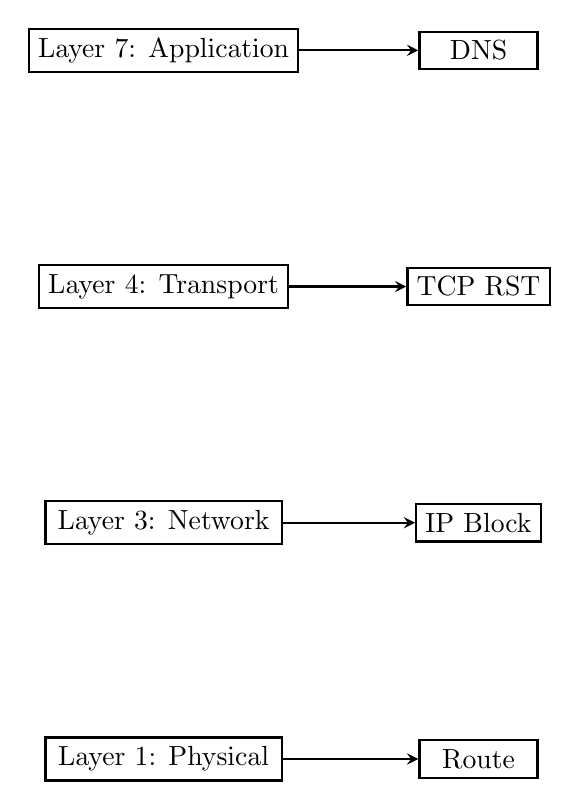
\begin{tikzpicture}[node distance=3cm,>=stealth,thick]
        \node (layer7) [draw, rectangle, minimum width=3cm] {Layer 7: Application};
        \node (layer4) [draw, rectangle, minimum width=3cm, below of=layer7] {Layer 4: Transport};
        \node (layer3) [draw, rectangle, minimum width=3cm, below of=layer4] {Layer 3: Network};
        \node (layer1) [draw, rectangle, minimum width=3cm, below of=layer3] {Layer 1: Physical};
        
        \node (dns) [draw, rectangle, minimum width=1.5cm, right of=layer7, xshift=1cm] {DNS};
        \node (tcp) [draw, rectangle, minimum width=1.5cm, right of=layer4, xshift=1cm] {TCP RST};
        \node (ip) [draw, rectangle, minimum width=1.5cm, right of=layer3, xshift=1cm] {IP Block};
        \node (route) [draw, rectangle, minimum width=1.5cm, right of=layer1, xshift=1cm] {Route};
        
        \draw[->] (layer7) -- (dns);
        \draw[->] (layer4) -- (tcp);
        \draw[->] (layer3) -- (ip);
        \draw[->] (layer1) -- (route);
    \end{tikzpicture}
    \caption{Network filtering can occur at multiple OSI layers.}
\end{figure}

\subsection{DNS Pollution and Hijacking}

\textbf{How it works:}
\begin{itemize}
    \item DNS queries are typically unencrypted (plaintext).
    \item When a DNS query for a blocked domain is detected, the firewall intercepts it.
    \item Instead of forwarding to the real DNS server, it returns a fake IP address.
    \item This is called "DNS pollution" or "DNS hijacking."
\end{itemize}

\textbf{Why it's effective:}
\begin{itemize}
    \item Very resource-efficient (minimal network overhead).
    \item Blocks most users who don't understand DNS.
    \item Works before any connection is established.
\end{itemize}

\textbf{How to detect:}
\begin{itemize}
    \item Compare DNS results from different DNS servers (8.8.8.8, 1.1.1.1).
    \item Use encrypted DNS (DNS over HTTPS/TLS).
    \item Check if resolved IPs are actually reachable.
\end{itemize}

\subsection{IP and Port Blocking}

\textbf{Route Nullification (Blackhole Routing):}
\begin{itemize}
    \item Firewalls can configure routers to drop packets to specific IP addresses.
    \item This is done by creating "null routes" or "blackhole routes."
    \item Packets are routed to a "blackhole" interface that discards them.
    \item Very efficient: packets are dropped before leaving the local network.
    \item This is why some IPs are unreachable even though DNS resolution works.
\end{itemize}

\textbf{Port Blocking:}
\begin{itemize}
    \item Specific ports (e.g., common VPN ports) can be blocked.
    \item Often combined with IP blocking for comprehensive filtering.
    \item Some firewalls block entire IP ranges (e.g., all of Google's IPs).
\end{itemize}

\subsection{Deep Packet Inspection (DPI) and Protocol Recognition}

\textbf{Keyword Filtering:}
\begin{itemize}
    \item Firewalls can inspect unencrypted traffic (HTTP, FTP, SMTP).
    \item When forbidden keywords are detected, TCP RST packets are sent to both sides.
    \item This terminates the connection immediately.
    \item Works because these protocols send data in plaintext.
\end{itemize}

\textbf{Protocol Fingerprinting:}
\begin{itemize}
    \item Different protocols have distinct "fingerprints" (handshake patterns, packet sizes, timing).
    \item Firewalls can identify protocols even if content is encrypted:
    \begin{itemize}
        \item OpenVPN: Specific handshake pattern
        \item PPTP: Distinct packet structure
        \item HTTP Proxy: CONNECT method pattern
        \item SOCKS5: Specific handshake sequence
    \end{itemize}
    \item Once identified, connections can be blocked or throttled.
\end{itemize}

\textbf{TLS Fingerprinting:}
\begin{itemize}
    \item Even encrypted TLS connections have identifiable characteristics.
    \item TLS handshake includes unencrypted metadata (cipher suites, extensions).
    \item Some implementations have unique fingerprints.
    \item Vulnerabilities in specific versions can be exploited for detection.
\end{itemize}

\subsection{TCP Reset (RST) Attacks}

\textbf{How TCP RST works:}
\begin{itemize}
    \item When a firewall detects forbidden content or protocol:
    \begin{enumerate}
        \item Firewall sends TCP RST packet to client (spoofed as server).
        \item Firewall sends TCP RST packet to server (spoofed as client).
        \item Both sides think the other disconnected.
        \item Connection is terminated immediately.
    \end{enumerate}
    \item This is why you might see "Connection reset by peer" errors.
\end{itemize}

\textbf{Why it's effective:}
\begin{itemize}
    \item Works on established connections (not just new ones).
    \item Very fast (connection drops immediately).
    \item Hard to distinguish from legitimate connection failures.
\end{itemize}

\subsection{Why Endpoints May Fail Even Outside Restricted Regions}

Even if you're outside regions with network filtering, endpoints can still fail for several reasons:

\subsubsection{Server-Side Restrictions}

\begin{itemize}
    \item \textbf{Geographic IP Filtering}: Servers may only accept connections from specific regions.
    \item \textbf{Whitelist-Based Access}: Some VPN servers only allow connections from other VPN servers.
    \item \textbf{Rate Limiting}: Servers may block direct connections but allow proxy connections.
    \item \textbf{Port Restrictions}: Servers may only accept connections on specific ports or from specific IPs.
\end{itemize}

\subsubsection{Protocol Requirements}

\begin{itemize}
    \item \textbf{Protocol-Specific Handshakes}: VMess, Shadowsocks, and other protocols require specific handshakes.
    \item \textbf{Simple TCP tests fail}: A basic TCP connection test can't perform the required protocol handshake.
    \item \textbf{Authentication Required}: Many protocols require authentication before accepting connections.
    \item \textbf{Encryption Keys}: Connections may require specific encryption keys or certificates.
\end{itemize}

\subsubsection{Network Path Issues}

\begin{itemize}
    \item \textbf{Intermediate Firewalls}: Your ISP or intermediate networks may block certain IPs or ports.
    \item \textbf{Routing Problems}: Network routing issues can prevent packets from reaching the destination.
    \item \textbf{Server Downtime}: The endpoint server may be down or overloaded.
    \item \textbf{Maintenance}: Servers may be temporarily unavailable for maintenance.
\end{itemize}

\subsubsection{Why Direct TCP Tests Fail But Proxy Works}

This is a common scenario:

\begin{enumerate}
    \item \textbf{Direct TCP test fails}: Simple TCP connection to endpoint times out or is refused.
    \item \textbf{But proxy works}: When connecting through a properly configured proxy client, it works.
    
    \textbf{Why?}
    \begin{itemize}
        \item Server may only accept connections with proper protocol handshake (VMess, Shadowsocks, etc.).
        \item Server may require connections from specific IP ranges (other VPN servers).
        \item Server may rate-limit direct connections but allow proxy connections.
        \item The proxy client performs the required protocol handshake and authentication.
    \end{itemize}
\end{enumerate}

\subsection{Interpreting Diagnostic Results}

When you see connection failures, consider:

\begin{itemize}
    \item \textbf{DNS Resolution Works}: Hostname resolves to IP → DNS is not the problem.
    \item \textbf{Routing Works}: Traceroute shows packets are being routed → Network path exists.
    \item \textbf{TCP Connection Fails}: SYN sent but no SYN-ACK received → Possible causes:
    \begin{itemize}
        \item Firewall blocking (intermediate or server-side).
        \item Server not accepting direct TCP connections (requires protocol handshake).
        \item Port is closed or service is down.
        \item Geographic restrictions.
    \end{itemize}
    \item \textbf{Proxy Test Fails}: Local proxy not available → Need to start proxy client first.
\end{itemize}

\subsection{Best Practices for Endpoint Testing}

\begin{enumerate}
    \item \textbf{Test DNS First}: If DNS fails, nothing else matters.
    \item \textbf{Test Routing}: Verify packets can reach the destination network.
    \item \textbf{Test TCP}: Check if basic connectivity works.
    \item \textbf{Test Through Proxy}: If direct fails, test through properly configured proxy.
    \item \textbf{Check Protocol Requirements}: Ensure you're using the correct protocol and authentication.
    \item \textbf{Consider Geographic Restrictions}: Some endpoints may only work from specific regions.
\end{enumerate}

\section{Further Reading}

\begin{itemize}
    \item RFC 791: Internet Protocol (IP)
    \item RFC 793: Transmission Control Protocol (TCP)
    \item RFC 2661: Layer Two Tunneling Protocol (L2TP)
    \item WireGuard Protocol Documentation
    \item VMess Protocol Specification (V2Ray)
    \item Shadowsocks Protocol Documentation
    \item DNS over HTTPS (DoH) and DNS over TLS (DoT) specifications
    \item TLS Fingerprinting research papers
\end{itemize}

